\chapter{Knot selection in compartmental spline models: osteoarthritis of the knee}
\label{applications-con_fit_splines}

Chapters~\ref{applications-splines_knot_loc} and
~\ref{applications-priors_knots_select} demonstrated the importance of
knot selection in spline models for sparse, noisy data. In this
chapter, we return to this point in the context of compartmental
models where the age-specific hazards are represented by splines and
the parameter of primary interest, prevalence, comes from the solution
to a system of differential equations based on these splines. In this
setting, modeling decisions about the knot locations for one parameter
affect the estimates for all the other parameters as well.  The
compartmental model for osteoarthritis of the knee provides a
demonstration of this.

Osteoarthritis (OA) is a joint disorder that affects joint cartilage and
underlying bone.  OA causes pain in the joints and limits movement.
OA of the knee is common and causes significant
morbidity, particularly in the
elderly. \cite{felson_epidemiology_1988, felson_incidence_1995}
Systematic review yielded $602$ data points representing $27$ countries
in $10$ GBD 2010 Study regions.

Since OA of the knee is exceedingly rare in young adults, expert priors inform the
model that the onset of the disease does not start before age 30.  The
number and location of knots in the incidence rate after this minimum
age of onset determine critical features of the model. As shown in
figure~\ref{fig:app-oa knee knots}, it is important to have enough
knots to represent the rapid change in age-specific incidence.
However, knot selection in incidence also affects estimates of
prevalence and excess mortality.

    \begin{figure}[h]
        \begin{center}
            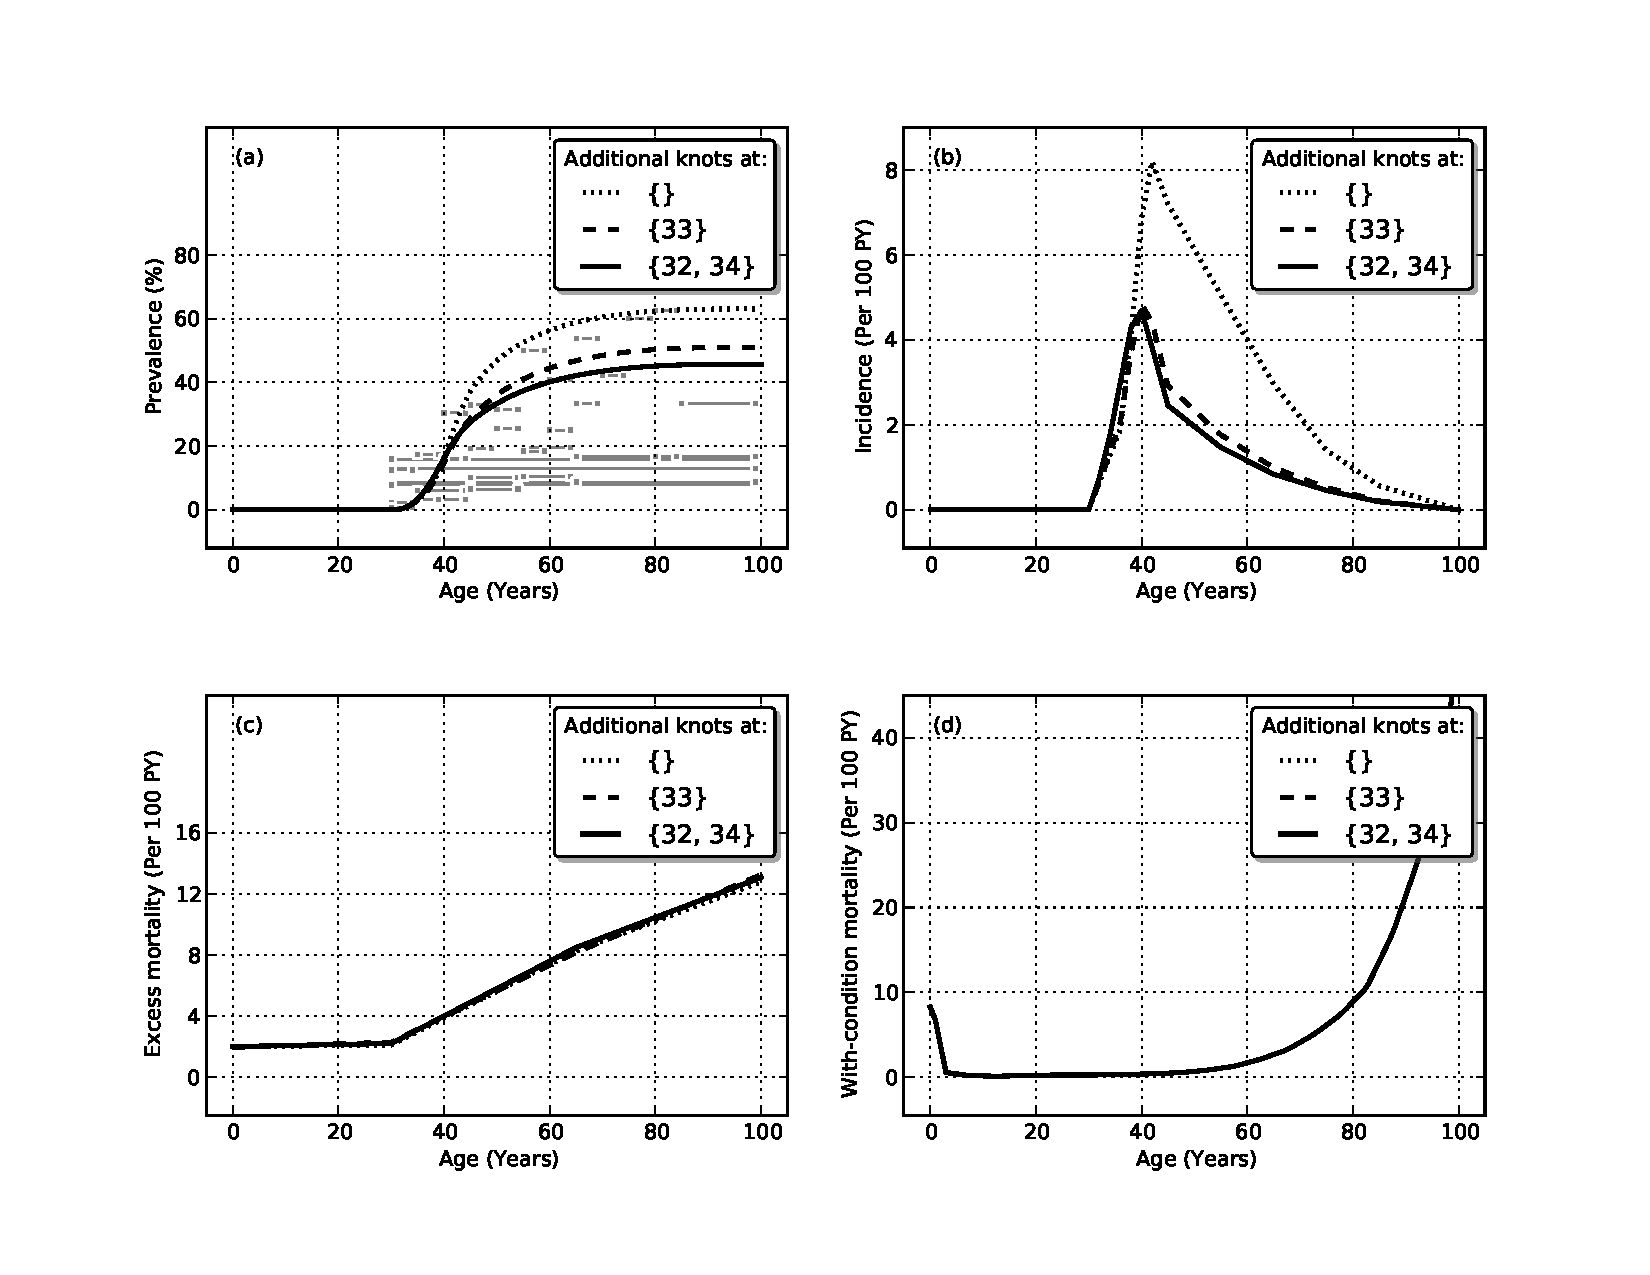
\includegraphics[width=\textwidth]{oa_knee-knots.pdf}
            \caption{Knot selection between the ages of 30 and 99
              plays an important role in the estimates of
              (a) prevalence, (b) incidence, and 
              (c) excess mortality
              for Western European females
              with OA of the knee in 2005.  The
              incidence rate of all models has knots at \{0, 30,
              40, 45, 65, 100\}.  Between the ages
              of 30 and 40, the models have either no additional knots \{\} or additional knots at \{35\}
              or \{31, 35\}.}
            \label{fig:app-oa knee knots}
        \end{center}
    \end{figure}

The model is also sensitive to assumptions about the epidemiological
profile, expressed in the model as expert priors.  Figure
~\ref{fig:app-oa knee priors} compares assumptions about OA of the knee
incidence.  A prior that requires zero incidence at ages greater than
$99$ implies that incidence decreases with age.  In other words, after a
certain age, if OA of the knee has not developed, it is unlikely it ever
will. Without this prior, incidence increases with age.  The logic
requirement of internal consistency in the compartmental model means
that prevalence estimates are also affected, as shown in figure
~\ref{fig:app-oa knee priors}.  When incidence is unrestricted,
prevalence has a very different age pattern than when incidence is
restricted.

    \begin{figure}[h]
        \begin{center}
            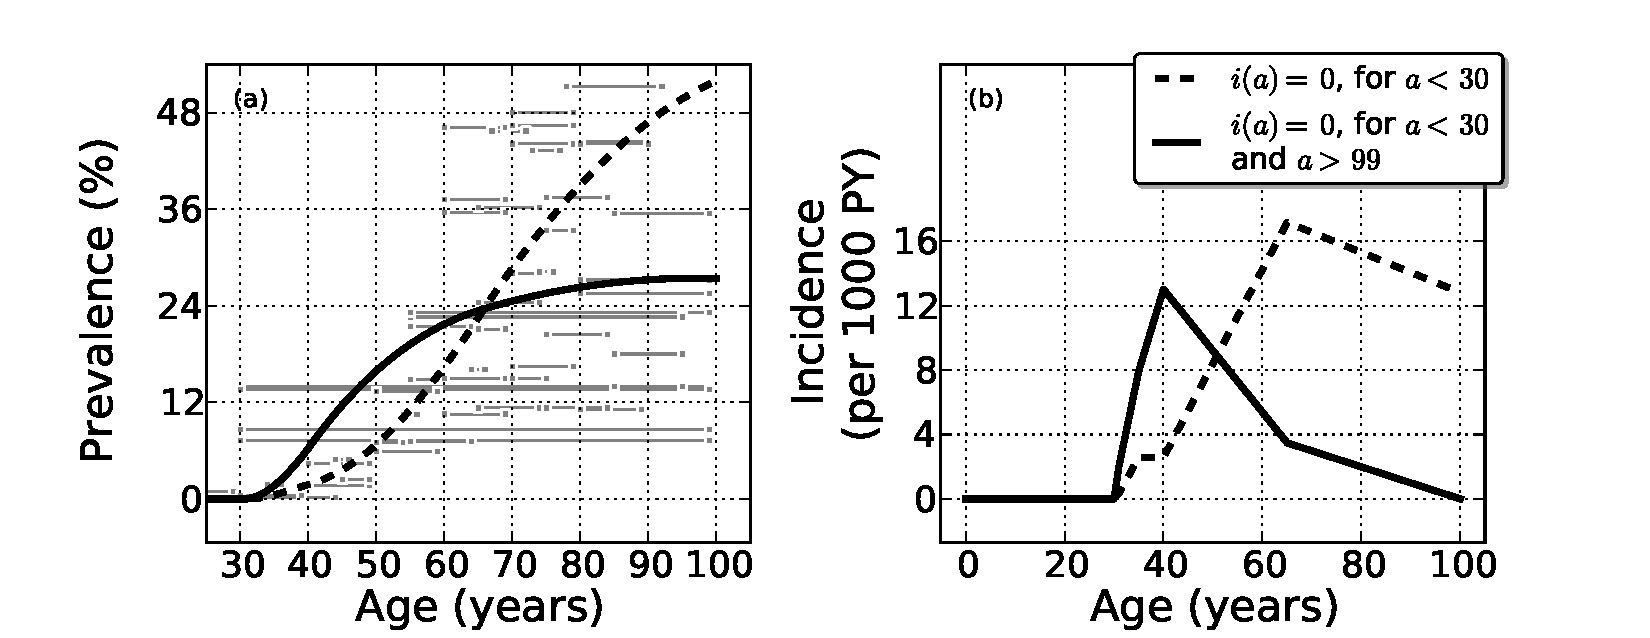
\includegraphics[width=\textwidth]{oa_knee-i_prior.pdf}
            \caption{A comparison of (a) prevalence and (b) incidence estimates
              for Western European females
              with OA of the knee in 2005 with and
              without a prior stipulating no onset of the disease in
              ages greater than $99$ using a compartmental model.}
            \label{fig:app-oa knee priors}
        \end{center}
    \end{figure}

Knot selection in compartmental models can be an influential part of
the model.  The logic requirement of internal consistency means that
modeling decisions for one parameter affect all parameters.  Knot
selection had a substantial effect on the estimates, although it can
be minimized by increasing the number of knots included in the model.
Likewise, informative priors on incidence drastically modified other
parameter estimates.  The influence of priors in compartmental
modeling is elaborated further in the following chapter.
